\chapter{Background}\label{ch:baseline}%

\section{Goal-oriented Requirements Engineering}

Goal-oriented requirements engineering captures the intentionality behind system requirements. More than just presenting the \textit{what} and the \textit{how} of a system-to-be, it provides the justification for each requirement, that is, they also present the \textit{why}. Through a directed graph tree that begins with a root goal, goals are connected trough decomposition links. Root and higher level goals are related to strategical concerns, while lower level and leaf-goals are related to technical and operational features of the system. 

The main purpose of a goal model is to support the early process of RE, including the elicitation of social needs and dependencies, the actors involved in delivering functionalities and resources, the decomposition of higher-level goals into more granular and detailed requirements chunks, the operationalization through means-end tasks and finally the comparison between different alternatives for the system-to-be. A goal model is said to be valid and complete if it follows all its syntactic rules and if all system goals are either decomposed, delegated to other actors or fulfilled by operational system tasks. 

Frameworks and methodologies like the i*, KAOS and TROPOS represent the foundations for the goal model analysis used by a variety of other proposals~\cite{Yu1996, Dardenne1993, Bresciani:2004}. Despite some syntax differences, most goal-oriented approaches share a set of common and more important concepts:
\bigskip

\Large{\underline{Intentional entities}}
\normalsize
\begin{itemize}

\item \textbf{Actor:} an entity that has goals and can decide autonomously how to achieve them. They represent a physical, social or software agent. E.g.: A patient, an emergency center, a doctor and a Mobile Personal Emergency System running in patient's smartphone.
\medskip

\item \textbf{Goal:} are actors' strategic interests. A goal with a clear-cut criteria for its satisfaction is called a hard goal. In opposition, softgoals has no clear-cut criteria for deciding whether they are satisfied or not and are usually represent non-functional requirements. E.g.: vital signs are monitored, emergency is detected, emergency center is notified (hard goals) and emergency awareness, precise assistance, feel supported (softgoals).
\medskip

\item \textbf{Task:} an operational means to satisfy actors' goals. E.g.: monitor temperature sensor, persist vital signs data, request emergency assistance.
\medskip

\item \textbf{Resource:} an information data or a physical resource that is generated or required by an actor.

\end{itemize}
\medskip

\Large{\underline{Relations}}
\normalsize
\begin{itemize}

\item \textbf{AND/OR Decomposition:} AND-decomposition (OR-decomposition) is a link that decomposes an actor's goal/task into actor's sub-goals/tasks, meaning that all (at least one) decomposed goals/tasks must be fulfilled/executed in order to satisfy its parent entity. 
\medskip

\item \textbf{Means-end:} a relation that indicates a means to fulfil an actor's goal through the execution of an operational task by the same actor.
\medskip

\item \textbf{Contribution link:} a positive or negative contribution between a given goal/task to a softgoal. Contribution links are used for deciding between alternative goals/tasks at design time (contribution analysis).
\medskip

\item \textbf{Dependency link:} a delegation of a goal, task or resource (\textit{dependum}) from an actor (depender) to another (dependee).

\end{itemize}

\section{TROPOS Goal-oriented Software Development Methodology}

TROPOS is a GORE methodology based on the i* framework~\cite{Bresciani:2004}. Its main improvement is the addition of new phases of requirements engineering, architecture and system design, namely:

\begin{itemize}

\item Late requirements engineering: Beyond the social dependency modelling with actors diagrams representing stakeholders and their needs in early requirements phase, a late requirements phase focuses on the system actor analysis. In this phase, system goals are inherited from stakeholders needs and represent both functional and non-functional requirements. Each goal has to be further decomposed in more granular sub-goals, delegated to other actors or to be fulfilled by means-end tasks. 
\medskip

\item Architectural design: In this phase, new actors representing sub-systems are created to fulfil different system goals. The idea is to shape the solution using a multi-agent architecture style instead of a monolithic system approach. Data and control interconnections are represented as dependencies.
\medskip

\item Detailed design: The last phase is characterized by the specification of agent capabilities and interactions though UML activity and sequence diagrams. Also, the implementation platform and other specific implementation details are addressed in order to directly map the design to system code.

\end{itemize}

%TROPOS implementation phase is out of the scope of this work as our objective is to improve the analysis and the solution that will be later implemented.

\section{Goals, Means and Contexts}

Context may be defined as the reification of the environment that surrounds the system operation~[FINKElSTEIN]. Contexts, as already stated, may not be static, but dynamic, and a system has no control over the context variation. Accordingly, a system must be able to support different contexts of operation without violating its functional and non-functional goals. To achieve this, systems must be able to monitor the state of its surrounding environment and take adaptive actions regarding the means used for fulfilling its goals.

%decide which alternative will be used regarding both the availability of that alternative and the optimization of non-functional requirements.

In GORE, dynamic contexts may affect what goals a system have to reach, the means available to meet them and also the quality achieved by each alternative[CGM]. Root goal and higher-level strategical goals are not contextualized as they represent the main purpose of a system [Finkelstein]. As these goals are decomposed in more granular sub-goals, a context condition may dictate:

\begin{enumerate}

\item If the goal is required for that context, limiting `what' a system should do;
\medskip

\item If a sub-goal or task is adoptable, limiting the `means' to fulfil a required goal;
\medskip

\item The positive, neutral or negative contribution of using some goal or task to another goal, usually a qualitative softgoal;

\end{enumerate}

The third effect is the main focus of this work, as it is related to non-functional metrics such as dependability attributes. Also, the other effects must also be considered by the verification model, including the variability at what goals are required at each context and what means are adoptable.

%the GORE contribution analysis that we aim to improve. In our proposal, we extend the concept of the context variation effect to non-functional metrics of goals and tasks - as the components used for concrete task execution may also be affected by context variations, e.g., the reliability of a sensor in different temperatures. 

\section{Variability in GORE}\label{sec:variability}

Given the possibility of an OR-decomposition in a goal model, more than one alternative can exist in terms of which subgoal should be achieved to satisfy its upper goal,  which subtask should be executed to satisfy its upper task or which task should be executed to satisfy its upper goal. Accordingly, multiple paths may lead to the satisfaction of the root goal. They are called alternative behaviours, or alternatives. 

Solving the variability problem in goal models have different meanings according to the development phase it takes place. 

\subsection{Design-time alternative selection}

At design time, multiple alternatives are elicited trough goal-oriented analysis, but not all are selected to be part of the system-to-be. In traditional GORE, contribution analysis is used for the the comparison of how each alternative contributes for one or more softgoals. Usually, only one alternative with the more positive contribution sum is selected for the system-to-be. Or, as in the simplistic example of Figure~\ref{fig:GORE_CA}, the decision should rely on the softgoals priority~\cite{Yu:2013}.

\begin{figure*}[h!]
\centering
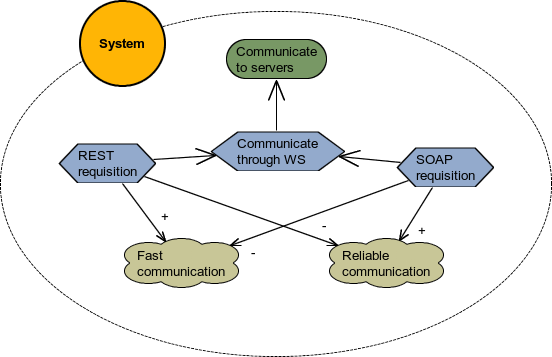
\includegraphics[width=0.6\textwidth]{imgs/GORE_CA.png}
\caption{Contribution analysis in TROPOS GORE.}
\label{fig:GORE_CA}
\end{figure*}

\subsection{Runtime analysis}

In contrast to the design-time variability in goal models, runtime variability depends on runtime input and must be preserved at runtime, i.e., variability is inherited by the solution design~\cite{Yu:2008}. Ali et al. investigates the influence of the context of operation on the decision of which alternative should be selected~\cite{Ali:2010}. For instance, if the traffic is jammed and the patient's condition is critical, an emergency chopper is selected for assistance in place of an ambulance.

In other cases, alternatives should be monitored and analysed in terms of non-functional metrics to decide which one is suitable or optimal for selection. Here, the context of operation does not directly defines the adoptable alternative, but its effect on the quality of each alternative is considered as a decision criteria. For instance, instead of only monitoring the traffic condition, a more complex analysis must estimate the probability of the ambulance to reach the patient in a restricted time unit as part of the analysis in a self-adaptation loop. 



%Our proposal aims to solve the variability in goal models at runtime through a probabilistic verification of system alternatives in multiple contexts of operation following both direct and indirect context effects over alternatives.

%to select the best alternative at design time for the system-to-be, or to select the best alternative at runtime for the system in operation. Both problems are related to how each alternative conforms to requirements in terms of softgoals and non-functional metrics and to the context of operation. At design time, estimation of NFR is conduced on the model of the system behaviour. 

%\subsection{Different paths, one context, one solution}
%
%Despite the elicitation of more than one path, only one alternative is kept at design time. Softgoals are generally used as criteria for the alternative selection~[i*, TROPOS, KAOS]. We extend TROPOS with a model-based verification of  non-functional constraints. Verification should point out at design time:
%
%\begin{enumerate}
%
%\item Which alternative conforms to the non-functional metrics associated to the goal model. 
%\medskip
%
%\item The best alternative given one or more metrics. In the last case, a multi-criteria approach should decide which alternative will be selected for the system-to-be.
%
%\end{enumerate}
%
%\subsection{Different paths, multiple contexts, multiple  solutions}
%
%A system affected by context variation may have to select different alternatives for different contexts, justifying variability in the system-to-be design. Solving variability becomes more complex as for each context a different alternative may provide the best contribution to softgoals and achieve higher values for non-functional metrics. 
%
%In our work, variability solving for multiple contexts involves an iterative verification in which contexts are analysed for all adoptable alternatives. At least one alternative must be able to fully satisfy both functional and non-functional requirements of the system.

%The later corresponds to the family verification of a dynamic software product lines~[GENAINA].

\section{Dependability Analysis}

The concept of dependability is related to dependence and trust as well as the ability of a system to avoid failures that are more frequent and more severe than certain threshold~\cite{Laprie2004}. According to Avizienis et al., dependability encompasses the following attributes: 

\begin{itemize}

\item Availability: readiness for correct service.
\medskip

\item Reliability: continuity of correct service.
\medskip

\item Integrity: absence of improper system alterations.
\medskip

\item Safety: absence of catastrophic consequences on the user(s) and the environment.
\medskip

\item Maintainability: ability to undergo modifications and repairs.
\medskip

\end{itemize}

%Correctness is opposed to failures. 

A holistic dependability specification has to include not only the software operation, but also the NFR for which that operation is meant. Non-functional requirements are an important factor to decide the acceptable frequency and severity of a software or hardware failure.

A failure is a perceived deviation from system expected behaviour that may have variable degrees of consequence on the user(s) and the environment. These failures are caused by specification faults or specification violations. In the first case, requirements and behaviour models fails to describe the system: either the goals or the means to fulfil then are incorrect, inappropriate or incomplete. In the second case, software or hardware behaviour did not follow its specification due to a natural phenomena, a human-made fault, a malicious fault or an interaction fault~[AVIZIENIS].

%Avizienis et al. also characterizes a failure according to four viewpoints. For this work, failure domain and failure consequence are important as they define .

The scope of this work is restricted to specification violations, i.e., we assume that a system specification is complete and consistent. Failures are restricted to anomalous behaviour of the components participating in the execution of system tasks, including technical components and human actors. Regarding the different means to attain dependability, our proposal consists of a fault forecasting as part of the analysis in a self-adaptation feedback loop.

%, i.e., we focus on the dependability analysis and the estimating metrics related to dependability and assuring their conformance to the dependability constraints associated to the goal model. 

%
%At early project phases, hazard resolution may involve simply getting more information about hazards or generating alternative design solutions~\cite{Leveson:1995}. In our work, we have used a qualitative means to analyse the dependability to be delivered by goals of a certain system taking into account contextual effects. Our approach improves the understanding of systems fault-causality effect and the identification of best approaches to reduce risk or even determine rates for safety or system level functional failure. Moreover, dependability requirement analysis cannot be accurately fulfilled without taking into account the context under which the system will operate.
%
%
%Avizienis et al \cite{Laprie2004} proposed a failure classification taxonomy with four viewpoints characterizing failures. In our approach, we use two categories: domain and consequence. We use the domain category to distinguish \textit{content} failures from \textit{timing} failures:
%
%\begin{itemize}
%
%\item{\textbf{Content failure}: When the content of the information delivered by a system task deviates from its specification}
%
%\item{\textbf{Timing failure}: When the time of arrival or the duration of the information delivered by some system task deviates from its specification}
%
%\end{itemize}
%
%The consequence of failures enables the definition of failures' severity. Two limiting levels are predefined and other intermediary levels could be defined for each case:
%
%\begin{itemize}
%
%\item{\textbf{Minor failure}: The harmful consequences of failures are limited or at most similar to the benefits provided by the correct operation of the system}
%
%\item{\textbf{Catastrophic failure}: The harmful consequences of failures are incommensurably higher than the benefits provided by correct operation of the system}
%
%\end{itemize}
%
%More details on the complete failure classification can be found in \cite{Laprie2004}. In our approach, a part of this taxonomy is used to guide the definition of the classes of failures severities and therefore the required level of dependability for different system goals. It also takes part in the identification of which dependability attribute is related to each contextual failure occurrence.  

\section{Probabilistic Model Checking and PRISM tool}

A model checking is a formal method that aims to automatically verify if a system model meets its specification for defined properties. Probabilistic model checking supports the verification of finite-state probabilistic models such as discrete-time Markov chain (DTMC), continuous-time Markov chain (CTMC) and Markov decision process (MDP). Different types of properties enables the verification of a vast range of non-functional metrics.

\subsection{PRISM tool}

The PMC technique used in this approach is supported by the PRISM model checker tool~[PRISM]. PRISM allows the modelling and analysis of systems which exhibit random or probabilistic behaviour. The decision of using PRISM as the probabilistic state-based model checker was due to the number of successful case studies that have used this tool, indicating its maturity~\cite{PRISM:pubs}.

%, and also due to its rich environment that is able to represent different kinds of probabilistic models and their evaluations. 

PRISM is suitable for different kinds of model evaluations depending on the abstraction level, the type of probabilistic model and the PCTL properties to be analysed. Both qualitative and quantitative analysis are available features in the simulation/verification environment. Other environments for modelling and PCTL property specification are also available in the tool.
  
\subsection{PRISM language}

PRISM language offers a rich set of constructs that may represent system modules, components and others architectural and design abstractions. Modules are the main structure in a PRISM model. Modules are composed of variable and commands. The first describe the finite states a module can be in. The former describe the behaviour of a module, i.e., the actions that may result in state transitions and are guarded by predicates which in turn can be composed of any variable in the model. Finally, labels are used for command naming and synchronization. A DTMC command in PRISM takes the following form: $$[action/label]<guard>\to<probability>:<update>;$$

\subsection{Dependability analysis with PMC}

As it will be explained in later sections, goal models may be extended with the behaviour specification required for the verification of some important dependability attributes. The objective is to anticipate non-functional dependability violations and to support the decision of which alternatives to use at runtime self-adaptation. A model checking technique should be used for dependability analysis as long as: 

\begin{itemize}

\item A formal system model may be built;
\medskip

\item Properties representing dependability attributes may be defined;
\medskip

\item The analysis overhead is justified, e.g., by its criticality.
\bigskip

\end{itemize}

\subsection{PARAM}

More recent PRISM versions also supports a parametric model checking, that is, instead of constant variables whose values must be initialized before verification, parameters replace these variables and a parametric formula is generated. Nonetheless, a previous PRISM extension tool named PARAM also provides parametric verification and has been further evaluated in case studies. For this reason, in this work have used PARAM for the generation of parametric formulas corresponding to a given probabilistic model and a PCTL property.

%That is, instead of providing the final evaluation for a given property, models may use parameters instead of initialized variables and the verification will output a parametric formula whose evaluation will estimate or verify the model for any valid combination of parameters values.

\section{Antlr Language Recognition Tool}

ANTLR or Another Tool for Language Recognition is a open source parser generator for reading, processing, executing or translating structured text or binary files. The main purpose is to automatically generate a parser for a custom language defined in a specific grammar language supported by the tool. The parser can then be imported in any version compatible JAVA project to build and walk parsed trees. 

As a result, any domain-specific language may be specified and then parsed using JAVA methods that will manipulate primitive attributes and objects according to what each parser rule and lexical term means for that language. In our proposal, ANTLR was successfully used to generate the parser for the regular expression language that specifies the behaviour of a runtime goal model (RGM) and for the context effect notations as proposed by the contextual goal model (CGM). Further details of the grammar with both parser rules and lexical terms is given in later section.

\section{Mobile Personal Emergency Response System}

The MPERS case study will be further detailed in later chapter as the proposed TROPOS extension is described with the MPERS goal models of requirements engineering development phases. As such, this section will cover some relevant aspects of this system that justify the use of our formal verification approach.

An emergency response system is a mission-critical system for which failures in achieving its main goals by the time they are required may lead to catastrophic consequences on users, i.e., on patients monitored by the system expecting to be promptly assisted in case of a medical emergency. Accordingly, any stakeholder that wishes to offer a service based on this system will have both ethical and contractual obligations regarding the safety of its product, that is, it must employ all means to prevent system failures.

MPERS is expected to have a high availability - as it must be ready to respond to an emergency that may happen at any time - and a high reliability - as an incorrect emergency response may lead to death or to costly false-positives. Integrity is a less critical attribute in this case, but must also be addressed as patient privacy may not be violated by disclosing his personal health or geolocation info to unauthorized persons. Maintainability is addressed, among others, by the use of a software development methodology and by the ability to update emergency rules remotely at runtime.

Environment changes is an important factor for MPERS, as the following conditions may change:

\begin{itemize}

\item The battery of the mobile device;
\medskip

\item The battery of vital signs sensors;
\medskip

\item The mobile signal used for data communication and for geolocation triangulation;
\medskip

\item The GPS signal used for geolocation;
\medskip

\item The health risk of the patient;
\medskip

\end{itemize}

For all these environment conditions, a context analysis as proposed by Ali et al. may define the rationale for context monitoring, i.e., for how each context condition may be asserted as true or false through the monitoring of environment information. Some contexts are mapped to single monitorable facts, like `GPS signal' and `battery life'. Other like `patient health risk' are composed of multiple facts in a propositional formula.


%Reliability verification of an Ambient Assisted Living System also based on body-area networks though PCM technique was explored by Fernandes~[Fernandes, 2012]. Reliability estimation demonstrates the non-determinism in the verification model that will result in an non-deterministic evaluation result. Moreover, PRISM cost/reward structures could be used for the verification of non-functional metrics such as power consumption. In this work, we limit the analysis to the reliability verification as part of a dependability analysis.

%It will be up to the analyst and stakeholders to define which type of probabilistic model and which PCTL properties must be analysed for each different system. Dependability attributes may be relevant for any sort of system, but are certainly important for systems with some criticality degree, i.e., for those whose failure could have severe or catastrophic consequences for the user(s) and for the environment.

